\chapter{全景漫游与人的关系}

\section{全景漫游的生理特性}
实现全景漫游与传统人机界面最大的区别在于全景漫游时的设备(包括 VR 眼镜或专用眼罩)距离人眼只有 2~3 公分距离,设备整体对人眼呈包裹状态。使用者仅可通过听觉和其他一些不够灵敏的感觉来感受外界环境,使用环境的舒适性就变得非常重要。

全景漫游与人体关联的感觉和生理运动大致有:视觉、听觉、平衡感等。如图\ref{fig:human_sence}。

\begin{figure}[htp]
\centering
\fbox{
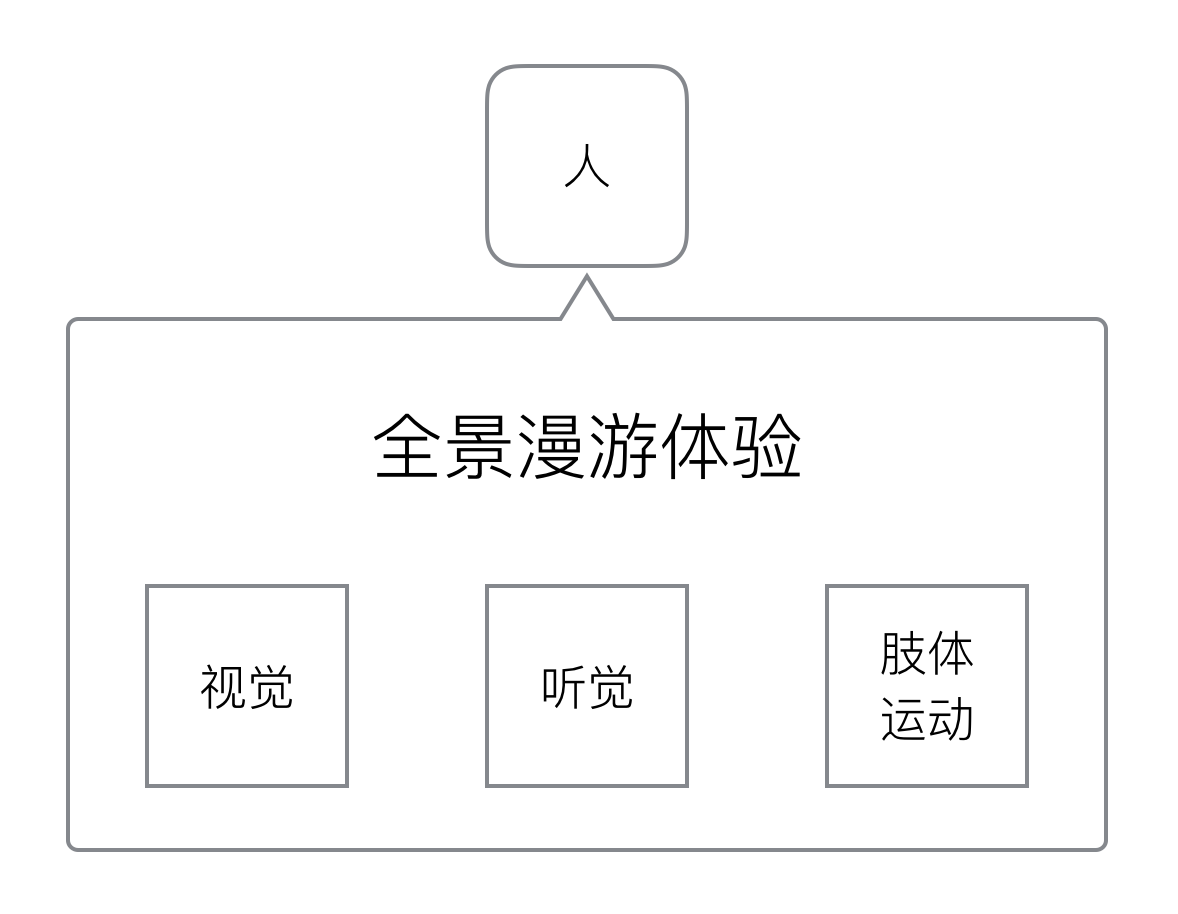
\includegraphics[width=.5\textwidth]{human_sence}
}
\caption{全景漫游与人体知觉}
\label{fig:human_sence}
\end{figure}

\subsection{全景漫游与视觉特征}
全景漫游对人体最大的刺激来源即是视觉刺激,其特征为距离眼睛距离近,色彩、明暗、动作变化等刺激较一般显示屏幕会更为剧烈。

\subsubsection{视角与视野}

人的视角是确定被看物尺寸范围的两端点光线射入眼球的相交角度。视角的大小与观察距离及被看物体上两端点的直线距离有关,其计算公式\ref{eq:angle}如下:
\begin{equation}
\alpha=2\arctan{\frac{D}{2L}}
\label{eq:angle}
\end{equation}

其中,$\alpha$ 为视角,用 $(^{\prime})$ 表示,即$(1/60)^{\circ}$单位;D 为被看物体上两端点的直线距离;L 为眼睛到被看物体的距离。
如果设眼球距镜片距离为 1.5cm,而镜片上一物体显示高度为 2cm,则带入公式可得\ref{eq:data}

\begin{equation}
\alpha=2\arctan{\frac{2cm}{2*1.5cm}}\approx 67.38 ^{\circ} = 2 \times 38.69^{\circ}
\label{eq:data}
\end{equation}

即上下视角各约为 $38.69^{\circ}$,查阅数据可知人在垂直平面的视野最大视区为视平线以上 $50^{\circ}$ 和视平线以下 $70^{\circ}$,颜色辨别界限为视平线以上 $30^{\circ}$,视平线以下 $40^{\circ}$。

由上述计算可知,在使用全景漫游设备观看场景时,假设高为 2cm 的显示物体在人视野中上部已超出颜色辨别界限,下部也已接近颜色辨别界限。物体上部比下部更接近垂直平面内的视野极限,如图\ref{fig:angle}。由此可知,全景漫游场景设计中应将主要元素置于屏幕中央,次要元素尽可能置于屏幕下方以便识别操作。同时,色彩丰富且饱和度高的元素也应置于视野中部,而一些操作类的元素则不应用过于丰富饱和的色彩缀饰,以免让使用者应难以分辨色彩而操作出错。

\begin{figure}[htp]
\centering
\fbox{
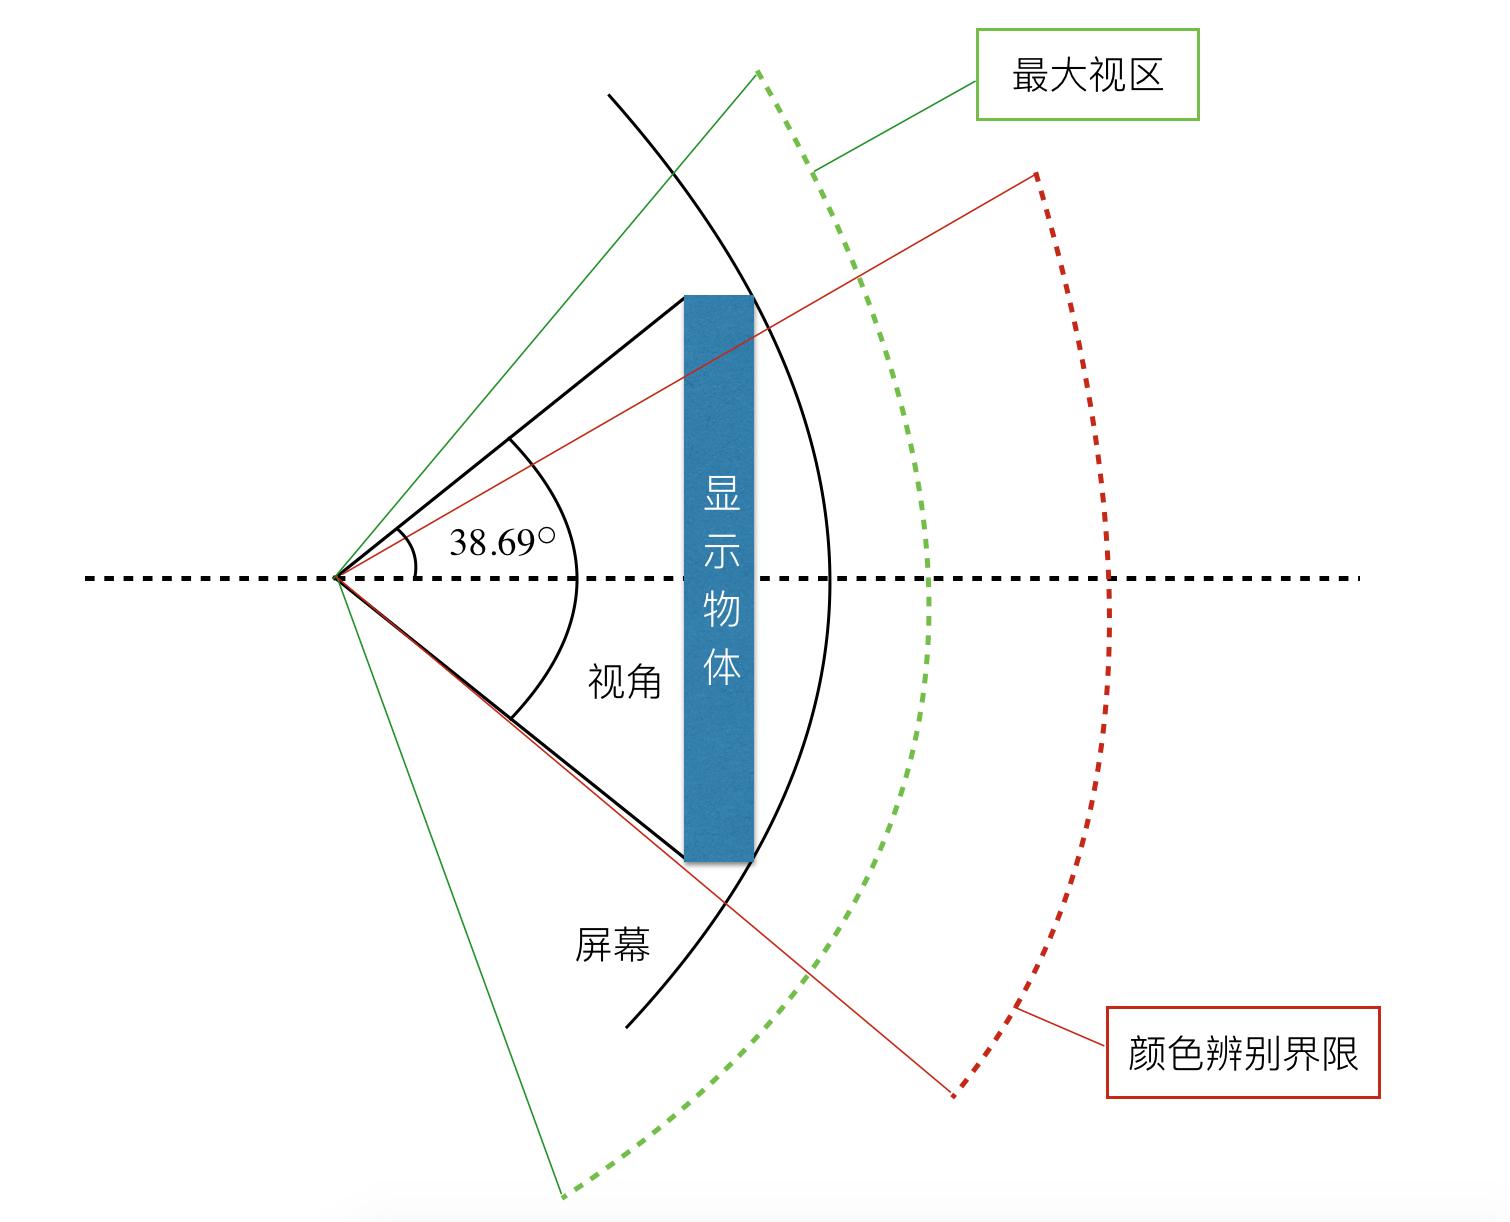
\includegraphics[width=.7\textwidth]{angle}
}
\caption{全景漫游中视野的角度关系}
\label{fig:angle}
\end{figure}

\subsubsection{视觉适应}

配戴全景漫游设备进行观察时,屏幕距眼球距离不足 2cm,属于视距过近状态,应当避免长时间操作,否则易引起眼睛疲劳。同时由于屏幕与眼球距离过近,屏幕亮暗对眼球刺激比通常工作环境更为强烈。当屏幕上场景切换间明暗变化过快时,人眼需要一定的适应时间才能正常分辨,但由于全景漫游设备等封闭性,无法较轻易地脱离这种明暗急剧变化的环境,则眼睛无法得到充足有效的适应时间,则很容易产生视觉疲劳,影响视觉能力。

\subsection{全景漫游与听觉}

全景漫游的视觉是主要人体感觉,但听觉是仅此于视觉的重要感觉,尤其是在视觉被全景场景完全包裹住的情况下。

现有全景漫游设备有的自带耳机设备,也有的需要自行配备耳机。但长远来看,配备耳机可能是必然的选择。因为人耳具有“方向敏感度”(或称“双耳效应”),即:声波在进入鼓膜时,受人体的反射、折射和衍射而扭曲变形,大脑能根据经验判断出声源的方位和距离。而前文所说的“耳听八方”即说的是这种能够重建场景音效的能力。

\subsubsection{双耳效应}
为了“制造”出能够“蒙骗”大脑使其误以为使用者身处虚拟场景中的体验,大致方向是重建出空间任意一点至双耳处的滤波器函数。我们不必去关心空间中某一点的声波是如何传播到人耳中的,只需要将该点声波信号经过滤波器便可以得到它在人耳处的声波信号,如图\ref{fig:hrtf}。而这个信号是可逆的,即被人耳捕捉到之后便由大脑还原成相应位置的“声信号”,从而达到“欺骗”大脑的目的。这个领域的研究对象叫做 HRTF(Head Related Transfer Function):头相关变换函数,是一种音效定位算法。但每个人的听觉能力都是不同的,所以 HRTF 对人类整体并没有通解,而只有对于人类个体经过反复实验测试后的特解。

\begin{figure}[htp]
\centering
\fbox{
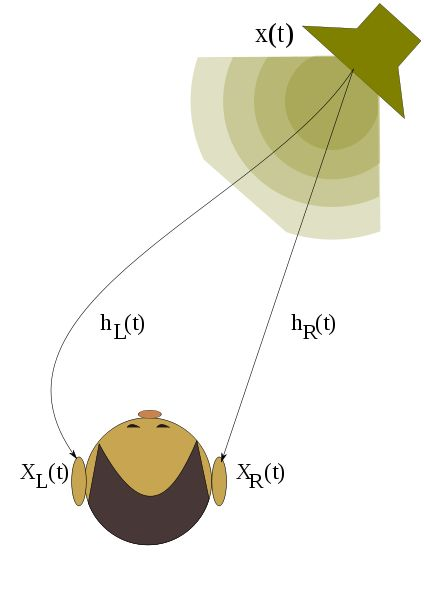
\includegraphics[width=.4\textwidth]{hrtf}
}
\caption{头相关变换函数 HRTF}
\label{fig:hrtf}
\end{figure}

国内外已有厂商根据相关理论设计并制作出了 VR 耳机,可配合 VR 眼镜使用,也可独立使用,它会追踪使用者的姿态、位置变化等,进而计算并还原出模拟三维场景内的声音分布,让使用者仿佛置于真实的场景之中。

\subsubsection{视觉的「补充」}
虽然声音不是可视化领域的研究重点,但良好的听觉体验的确有利于信息渠道的建立。视觉与听觉互为补充、相互作用、最终是人的知觉更为敏锐而准确。可以设想以下场景:「用户配戴全景漫游头盔进行一场探险类的游戏,用户扮演的主人公正在探索未知的世界,正当主人公小心翼翼地穿过一片沼泽时,后方突然传来了一声尖叫…… 」如图\ref{fig:audio-source}看不见的事物通过音效来表现,可以提升场景所渲染出的气氛效果。听觉与视觉不同,不受方向影响,能够用来表现一些视觉上无法做到的特殊效果。

\begin{figure}[htp]
\centering
\fbox{
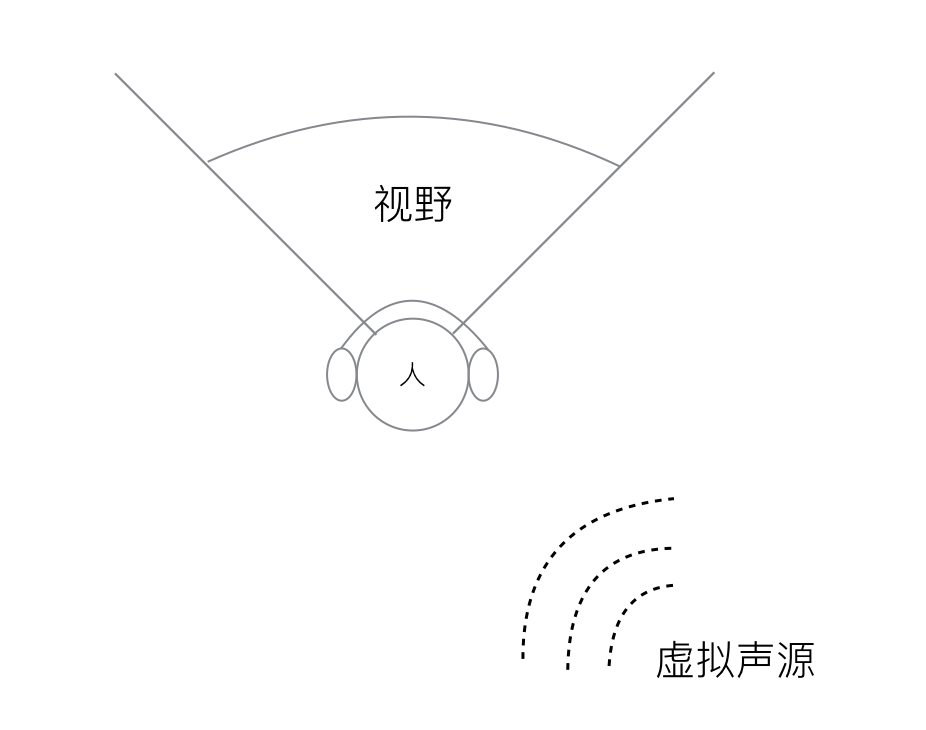
\includegraphics[width=.5\textwidth]{audio-source}
}
\caption{用音效来表现「看不见」的事物}
\label{fig:audio-source}
\end{figure}

\subsection{全景漫游与其他感觉}
众所周知的是,人之所以可以站立行走、骑行脚踏车或进行高空作业依赖的是人与生俱来并在后天不断磨合的平衡感。平衡感由内耳的淋巴液控制,同视觉相互配合,使人能安全地四处走动。而在全景漫游过程中,人的视觉几乎全部集中在眼前的屏幕上,即很难看到外界真实的场景,故视觉此时便难以匹配内耳中内淋巴液流动引起的细胞兴奋,对人来说就是平衡感的缺失。失去平衡感会使人晕眩,严重时会使人倾倒,有造成意外伤害的可能,故在进行全景漫游时应尽可能减少乃至避免对平衡感造成的影响。

维持平衡感有两种方式,一种是降低运动的速率(即减小在全景漫游中需要运动的强度)视为主动维持平衡感,另一种是通过某些手段来减少视觉或其他感觉中平衡感的减少,即运动补偿,可视为被动维持平衡感。

现有全景漫游设备部分带有陀螺仪、部分利用手机内置陀螺仪用以感应方位信息,可做运动补偿以模拟人在环境中的运动,但人的眼球可以根据平衡来进行前庭—眼动反射 ( vestibulo-ocular reflex)控制眼球作补偿性运动,使之匹配头部的转向,以求维持人视野的稳定。这套机制在不戴全景漫游设备时可以正常运作,但在配戴了全景漫游设备后因眼镜视野与外界隔离,故设备与外界的运动匹配度就变得格外关键。

现有普通手机所内置的是微机电陀螺仪(MEMS),是利用物理学的科里奥利力,在内部产生微小的电容变化,通过测量电容,计算出角速度,从而判断物体转向和速度,这种芯片价格低廉,体积小巧,但缺点是因其电磁特性易受环境干扰,而且精度即使能够满足一般手机应用(如转屏、翻转等)但在更为精细的全景漫游的方位感应上还是显得力不从心。屏幕显示画面本身就有约 1/60s 即 16ms 左右的刷新时差,再加上陀螺仪反馈信息与实时状态也有偏差,两者累积后在使用者运动时画面很难及时更新至准确的位置上,容易造成失去平衡的感觉。甚至在人停止运动后,全景漫游设备错误地输出带有运动补偿的画面以致人眼误以为人体还在做运动,造成认知上的偏差,导致非运动状态下的感官刺激,这种刺激往往对使用者造成较长时间的影响,延续到使用完全景设备后的数分钟乃至若干小时后。

全景漫游技术的发展在维持人体平衡感方面尚有很大的发展空间,现有高端全景漫游设备即使是支持全方向漫游的平台也只允许使用者慢步使用,而运动补偿机制仍沿用着手机等终端的设计(大多数全景漫游设备并没有自己的陀螺仪,而是直接调取了与其连接的手机的重力感应接口)在需要高精度分辨的场合表现就达不到使用要求了。

\section{全景漫游与肢体动作}

全景漫游,其一是“全景”,其二则是“漫游”。漫游,意为随意游玩、漫无目的地行走。全景漫游的体验重在参与感的营造,用户不仅能够“身临其境”般地体验全景场景,更可以亲身参与其中,与场景中的虚拟事物进行互动。

\subsection{关节运动}

全景漫游人体主要运动可分解为躯干的平面运动和头部的转动,这两方面配合眼球的转动就构成了全景漫游中人个体在场景中的位移和转向,如图\ref{fig:act}。

\begin{figure}[htp]
\centering
\fbox{
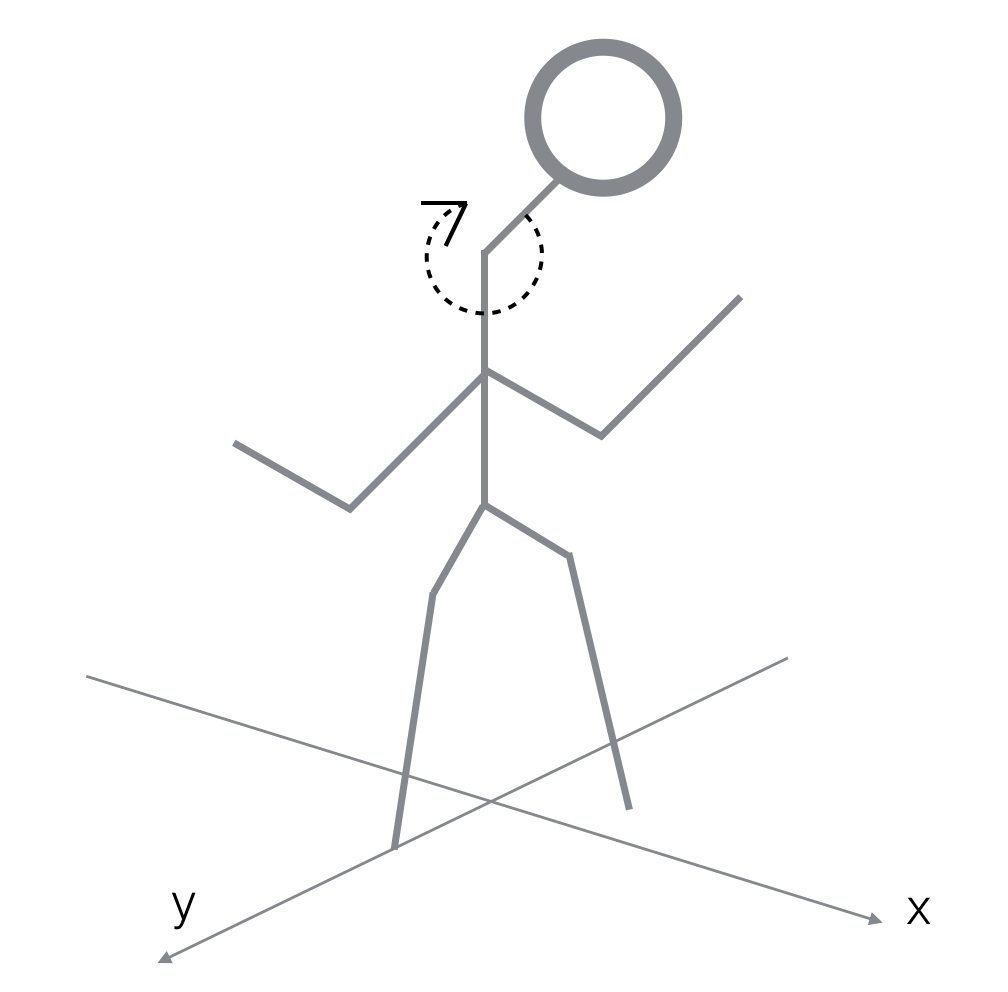
\includegraphics[width=.5\textwidth]{act}
}
\caption{躯干的平面运动与头部的转动}
\label{fig:act}
\end{figure}

但躯干的平面运动一般受场地的制约,并不是绝对的自由行进,而且由于人在看不到外界环境时处于一种对外界警惕的状态,实现行走不是全景漫游最优的运动方式。头部的转动则是一种比较好的选择,首先它的运动幅度较小,易于控制,其次头部转动也是人本能的反应,符合人对场景活动的预期。

人头部转动的形式有以下几种:低头与仰头、左歪与右歪、左转与右转。低头仰头的最大范围为 75°,另两种形式都为 110°,但低头舒适范围为 25°,仰头舒适范围为 12°。由此可得,全景漫游所用观看形式仍应以正面为主,辅以左右延展开的场景以供转头观察,这样可使人在舒适范围内使用全景漫游设备。同时,除主要场景外的功能部件也因设置在上下方向,以方便使用者通过低头仰头就可捕捉到所需要的部件。

同时,因为环境等不确定因素,易使用户丢失通过视觉等多种方式建立起的方位感。为避免方位感丢失对用户造成的迷茫,随时随地可以回到初始状态的功能也需处处设计在全景漫游中。

\subsection{手部活动}

漫游只是满足人观察的需求,需要与场景互动仍需要更多样化的操作形式。手势操作自然而然成了人控制的最佳选择,现有手柄、传感手套、指环甚至肌肉传感器可以作为全景漫游的输入装置。

\subsubsection{手:手柄}
通过手柄来体验场景可以说是最符合全景漫游现状的一种操作方式了,如图\ref{fig:handler}。无需过多说明,使用者会自然而然将手柄与游戏中呈现的自己的“双手”在脑海中联结起来。例如,简单的射箭游戏中,使用者在若干次尝试后就能“学会”通过左手握住手柄并保持,右手握住手柄并后拉来张开场景中的”弓“,如图\ref{fig:shoot}。手柄的优点是操作简便,其与全景漫游屏幕可类比成鼠标与计算机显示屏,但缺点是交互形式略微单一(摆动手臂,按下按钮等)。

\begin{figure}[htp]
\centering
\fbox{
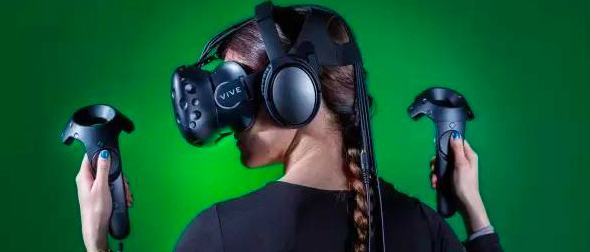
\includegraphics[width=.5\textwidth]{vr-handler}
}
\caption{用以全景漫游中操作的手柄}
\label{fig:handler}
\end{figure}

\begin{figure}[htp]
\centering
\fbox{
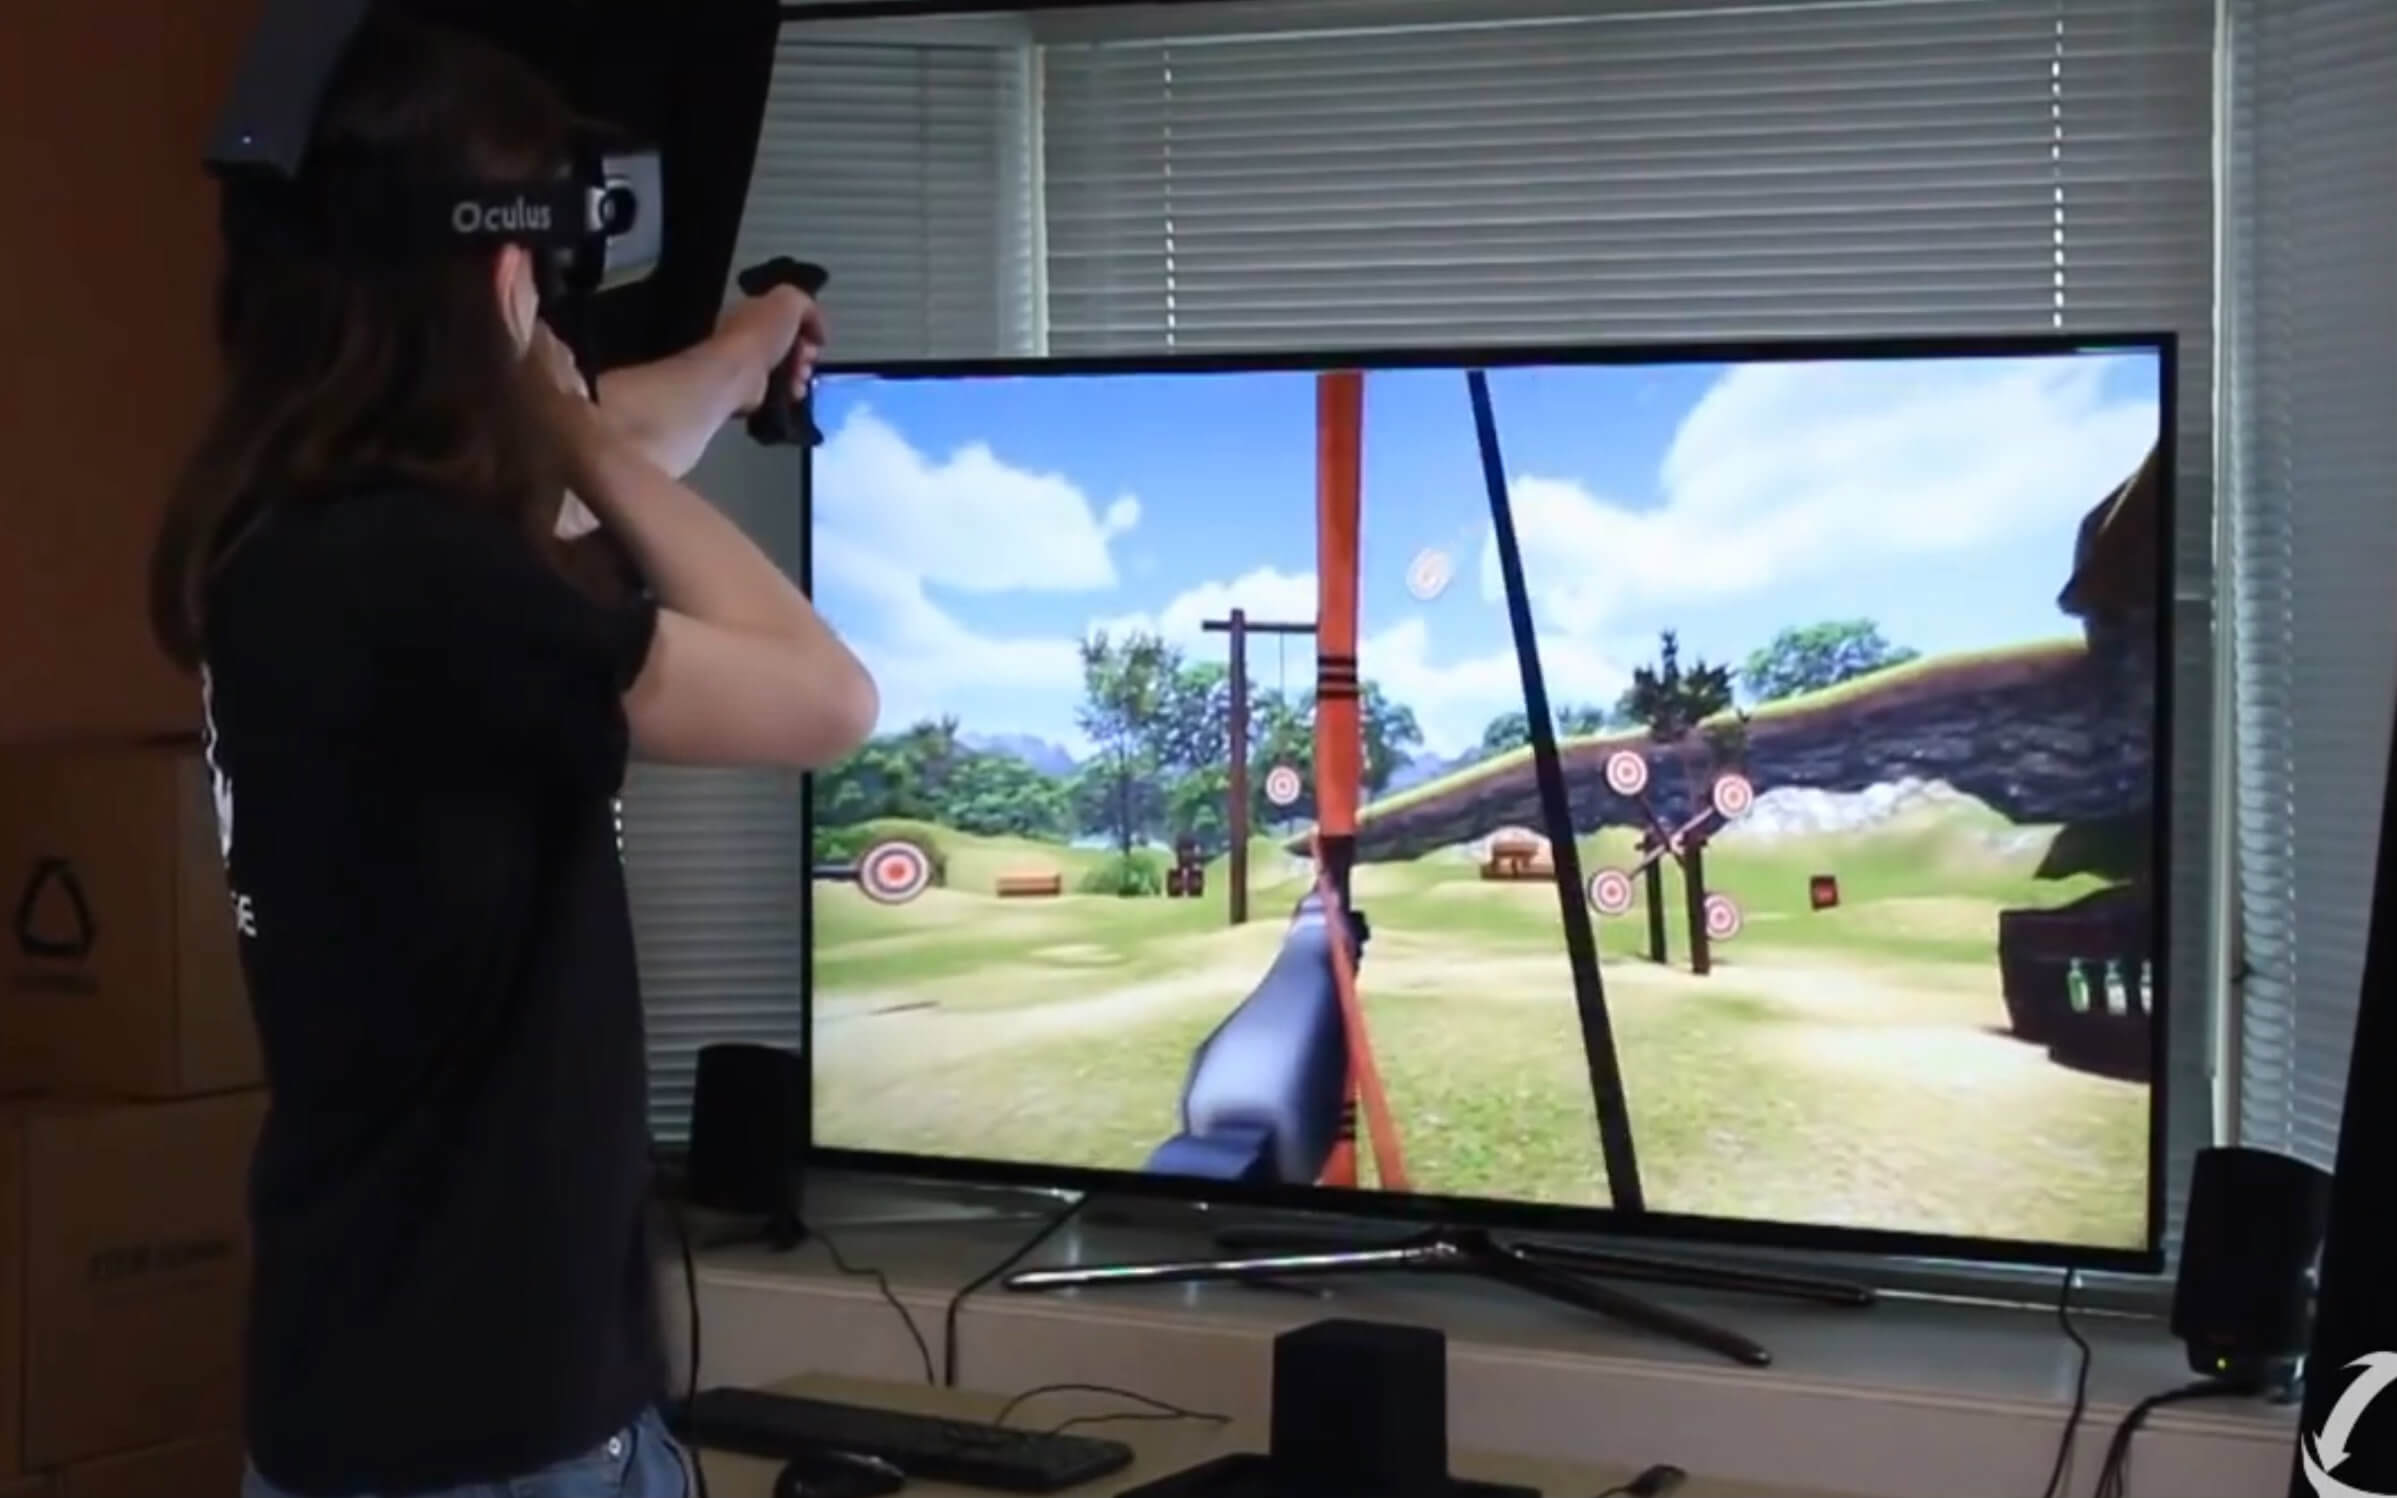
\includegraphics[width=.5\textwidth]{vr-shoot}
}
\caption{使用手柄控制全景漫游中的射箭动作}
\label{fig:shoot}
\end{figure}

\subsubsection{手指:传感手套}
手柄无法做到的操作形式之一是捕获手指的作用,而显然可知的是,人手进行各种动作时绝大部分操作都是通过手指来完成的,将人手指的操作追踪到系统中将极大地提高全景漫游中操作的便利性,如图。但目前手套类套件的局限性也是非常明显,比如手套相比手柄而言与手接触面积更大,在配戴时难免造成一定的不适应。而从控制计算而言,手套所需要的传感器数量将远远超过手柄,其开发相关的程序逻辑复杂性也会大大增加,故当前全景漫游配套手套尚未得到普及。

\begin{figure}[htp]
\centering
\fbox{
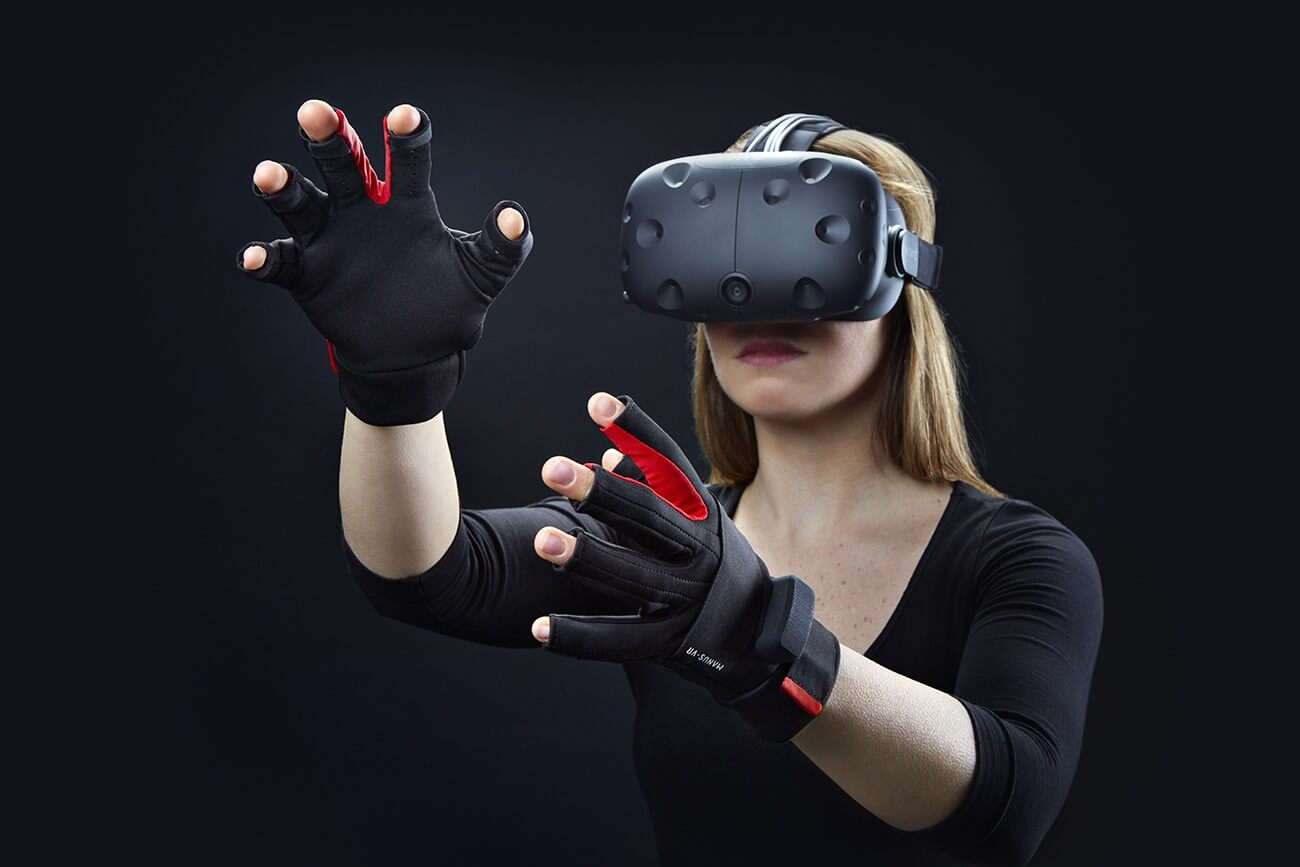
\includegraphics[width=.5\textwidth]{vr-gloves}
}
\caption{使用手套可在全景漫游中进行更为精细的操作}
\label{fig:gloves}
\end{figure}

\subsubsection{单个手指:指环}
指环作为手柄和手套的中间替代品,相比后两者而言,指环更为小巧。相比于操作手柄,通过指环与场景进行交互会更为简便,不必过于考虑把持手柄所带来的累赘感,指环如配合更为敏感的传感器或可实现相比手柄更为灵敏的操作,如图\ref{fig:ring}。相比手套而言,指环显得不易沾染污垢、细菌等,而且由于其又可作为配饰携带,拥有者会更倾向拥有一枚可以长期配戴的指环,而不是仅在全景漫游时可用的手套。


\begin{figure}[htp]
\centering
\fbox{
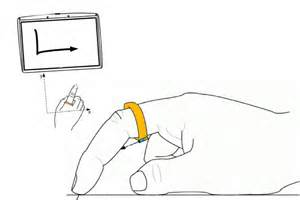
\includegraphics[width=.5\textwidth]{vr-ring}
}
\caption{配戴指环通过手指进行操作}
\label{fig:ring}
\end{figure}

\subsubsection{手部操控方式比较}

\begin{tabular}{|l|l|l|l|}
\hline
类别 & 手柄 & 手套 & 指环 \\
\hline
\end{tabular}
